\newpage
\section{Слабо неоднородные поля}
\subsection{Электрическое поле}
    Ограничимся рассмотрением сил, действующих на систему частиц в слабо неоднородном поле.
    Пусть имеется некоторая система частиц, заданная радиус-вектором $\vec{R}$ центра системы
    из которого до каждой $i$-й частицы проведён радиус-вектор $\vec{r}_i$. На каждую частицу действует поле $\vec{E}\brackets{\vec{R} + \vec{r}_i}$.
    Будем также считать, что $\abs{\vec{r_i}} \sim l$, то есть система имеет характерный размер $l$, причём $\frac lL \ll 1$, где $L$ --- так называемый
    масштаб неоднородности. Это выражение означает, что в границах системы поле меняется незначительно. Сила, действующая на систему, равна
    \[
        \vec{F} = \sum_i e_i \vec{E}\brackets{\vec{R} + \vec{r}_i}.
    \]
    Польуясь слабой неоднородностью, разложим поле $\vec{E}$ по градиентам (в ряд Тейлора):
    \[
        \vec{F} \approx \sum_i e_i \braces{\vec{E}\brackets{\vec{R}} + \brackets{\vec{r}_i \cdot \vec{\nabla}}\vec{E}\brackets{\vec{R}}} = 
        e\vec{E}\brackets{\vec{R}} + \brackets{\vec{d} \cdot \vec{\nabla}}\vec{E}\brackets{\vec{R}},
    \]
    где $e$ --- полный заряд системы, а $\vec{d}$ --- её дипольный момент:
    \[
        \vec{d} = \sum_ie_i\vec{r}_i.
    \]
    Если система электронейтральна, то есть суммарный заряд равен нулю, главную роль играет градиентное слагаемое,
    и сила действует на систему только в неоднородном поле.
    Найдём также момент сил, действующих на систему:
    \[
        \vec{K} = \sum_i \vecp{r_i}{F_i} = \sum_i \sqbrk{\vec{r}_i \times e_i\vec{E}\brackets{\vec{R} + \vec{r}_i}} \approx \sum_i \sqbrk{\vec{r}_i \times e_i\vec{E}\brackets{\vec{R}}} =
        \sqbrk{\vec{d} \times \vec{E}\brackets{\vec{R}}}.
    \]
\subsection{Магнитное поле}
    Теперь изучим слабо неоднородное магнитное поле. Вместо статической системы мы будем рассматривать систему стационарно движущихся частиц.
    В этом случае момент сил, действующих на систему, равен
    \[
        \vec{K} = \sum_i\vecp{r_i}{F_i} \approx \sum_i \frac{e_i}{c} \sqbrk{\vec{r}_i \times  \sqbrk{\vec{v}_i \times \vec{H}\brackets{\vec{R}}}}
    \]
    Перейдём к усреднённым за время (период) движения значениям:
    \begin{gather*}
        \vec{K} = \overline{\sum_i\vecp{r_i}{F_i}} = \sum_i \overline{\frac{e_i}{c} \braces{\vec{v}_i \dotp{r_i}{H} - \vec{H} \dotp{r_i}{v_i}}} = 
        \sum_i \overline{\frac{e_i}{c} \vec{v}_i \dotp{r_i}{H}} -\frac 12 \overline{\frac{d}{dt} \sum_i \vec{H}\dotp{r_i}{r_i}}.
    \end{gather*}
    Так как движение системы стационарное и финитное, величина $\abs{\vec{r_i}}^2 = \dotp{r_i}{r_i}$ ограничена. Значит, второе слагаемое обращается в нуль как
    среднее значение полной производной по времени от ограниченной функции:
    \[
        \overline{\frac{df}{dt}} = \lim_{T \rightarrow \infty} \frac 1T \int\limits_0^T dt \frac{df}{dt} = \lim_{T \rightarrow \infty} \frac{f(T) - f(0)}{T} = 0.
    \]
    Далее, легко проверить, взяв производные, что
    \begin{equation}
        \sum_i \overline{\frac{e_i}{c} \vec{v}_i \dotp{r_i}{H}} = \frac 12 \overline{\frac{d}{dt}\sum_i \frac{e_i}{c}\vec{r}_i\dotp{r_i}{H}}
        + \frac 12 \overline{\sum_i\frac{e_i}{c}\vec{v}_i \dotp{r_i}{H}} - \frac 12 \overline{\sum_i \frac{e_i}{c} \vec{r}_i \dotp{v_i}{H}}. \label{big_thing}
    \end{equation}
    Аналогично, первое слагаемое в выражении (\ref{big_thing}) равно нулю как среднее производной по времени ограниченной функции. Два других слагаемых
    можно представить в виде двоёного векторного произведения:
    \begin{gather*}
        \frac 12 \overline{\sum_i\frac{e_i}{c}\vec{v}_i \dotp{r_i}{H}} - \frac 12 \overline{\sum_i \frac{e_i}{c} \vec{r}_i \dotp{v_i}{H}} =
        \overline{\sum_i\frac{e_i}{2c} \sqbrk{\vec{H} \times \vecp{v_i}{r_i}}} = \\
        = \overline{\sum_i \frac{e_i}{2c}\sqbrk{\vecp{r_i}{v_i} \times \vec{H}\brackets{\vec{R}}}} =
        \vecp{m}{H}.
    \end{gather*}
    Величина $\vec{m} = \overline{\sum_i \frac{e_i}{2c}\vecp{r_i}{v_i}}$ называется \textit{магнитным моментом} системы.

    Точно таким же способом вычисляется средняя сила (задача №14):
    \[
        \vec{F} = \overline{\sum_i \frac{e_i}{c} \sqbrk{\vec{v}_i \times \vec{H}\brackets{\vec{R} + \vec{r}_i}}} = \dotp{m}{\nabla}\vec{H}.
    \]

\subsection{Прецессия Лармора}
    Рассмотрим достаточно важный случай системы заряженных частиц, в которой отношение массы каждой частицы к её заряду $m_i \big/ e_i$ одинаково для всех частиц.
    Магнитный момент этой системы равен
    \[
        \vec{m} = \frac 1{2c} \sum_i e_i \vecp{r_i}{v_i}.
    \]
    Положим $v \ll c$ --- нерелятивистский случай. При этом условии момент частицы $\vec{p}_i = m_i \vec{v}_i$, и магнитный момент частицы
    можно связать с механическим моментом $\vec{M} = \sum_i \vecp{r_i}{p_i} $ простой константой: 
    \[
        \vec{m} = \frac 1{2c}\sum_i \frac{e_i}{m_i}m_i\vecp{r_i}{v_i} = \frac{e_i \big/ m_i}{2c}\sum_i\vecp{r_i}{p_i} = g\vec{M}.
    \]
    Эта константа $g = \frac{e_i \big/ m_i}{2c}$ называется \textit{гиромагнитным отношением}.
    
    Поместим теперь рассматриваемую систему в центральное электрическое поле, например, создаваемое тяжелой частицей --- 
    атомным ядром с зарядом $Ze$, а также в однородное магнитное поле $\vec{H}$ (см. рисунок).

    \begin{figure}[h]
        \centering{
            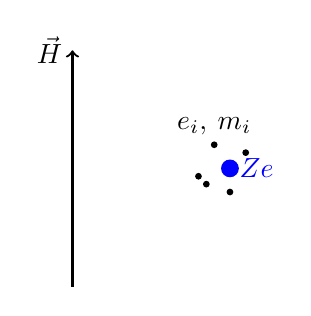
\begin{tikzpicture}
    \draw [->, thick] (0, 0) -- (0, 3) node [anchor = east] {$\vec{H}$};
    \filldraw [blue] (2, 1.5) circle (3 pt) node [anchor = west] {$Ze$};
    \filldraw [black] (2.2, 1.7) circle (1 pt);
    \filldraw [black] (1.6, 1.4) circle (1 pt);
    \filldraw [black] (1.7, 1.3) circle (1 pt);
    \filldraw [black] (2.0, 1.2) circle (1 pt);
    \filldraw [black] (1.8, 1.8) circle (1 pt) node [anchor = south] {$e_i, \: m_i$};
\end{tikzpicture}
        }
    \end{figure}

    Уравнение моментов для этой системы:
    \[
        \frac{d\vec{M}}{dt} = \vec{K} = \vec{K}_{\vec{E}} + \vec{K}_{\vec{H}}.
    \]
    Момент электрических сил $\vec{K}_{\vec{E}} = \sum_i \vecp{r_i}{F_{ei}}$ равен нулю, так как $\vec{F}_{ei} \parallel \vec{r}_i$.
    Остаётся только момент магнитных сил:
    \[
        \frac{d\vec{M}}{dt} = \vecp{m}{H} = g\vecp{M}{H} = \vecp{\Omega}{M},
    \]
    где $\vec{\Omega} = -g\vec{H} = -\frac{e}{2mc}\vec{H}$ --- частота прецессии вектора механического момента вокруг оси
    магнитного поля $\vec{H}$. Это явление называют \textit{ларморовской прецессией}, а величину $\vec{\Omega}$ --- \textit{ларморовской частотой}.